% Provenance (never printed): see sources/outline_sources.md (Year 1: litho-, bio- and
% chronostratigraphy; boundary stratotypes; mass extinctions as global markers; the
% international chart). Exercise and problem values in the Book 3 scratch calculator
% calc/ch24.py; the chart from figdata/bachelor-1/ics_chart.py (shared ics rows).
% The principles of relative dating, eras and periods are Book 1's (g7 geological-time) and
% are re-founded here. Mass extinctions belong to the biology series (recalled in prose);
% their Earth causes are the Year 2 volume's (phanerozoic-earth). Correlation of logs and
% unconformities are ch. 5's; facies ch. 21's; compaction ch. 23's. Radiometric dating is
% ch. 25's. Sequence stratigraphy, facies models and Walther's law are the Year 3 volume's;
% magnetostratigraphy too: prose pointers only. "Transgression" is explained in prose.
\chapter{L'échelle stratigraphique}\label{ch:b1:stratigraphic-scale}

Sur la plage d'Itzurun, à Zumaia sur la côte basque, les falaises sont faites de
minces bancs de calcaire et de marne, inclinés et répétés sur des centaines de mètres. À un
contact, là où un banc de calcaire pâle s'achève et où des marnes rouges commencent, un disque de bronze
frappé de quatre lettres est scellé dans la roche (figure ci-dessous). C'est un clou
d'or. Il fixe, pour la planète entière, l'instant où commence une division du
temps géologique --- l'\omterm{def:b1:stratigraphic-scale:chronostratigraphy}{étage} Sélandien. Une roche de Patagonie ou de
Sibérie est sélandienne si elle s'est déposée après l'instant enregistré à ce
contact et avant celui enregistré au clou suivant plus haut dans l'échelle. Ce chapitre
explique comment les géologues en sont venus à avoir besoin d'un tel repère~: trois façons
différentes de diviser un empilement de roches, les principes qui les ordonnent, les lignes qui relient
des coupes éloignées, et la charte internationale qui rassemble le résultat.

\begin{omfigure}
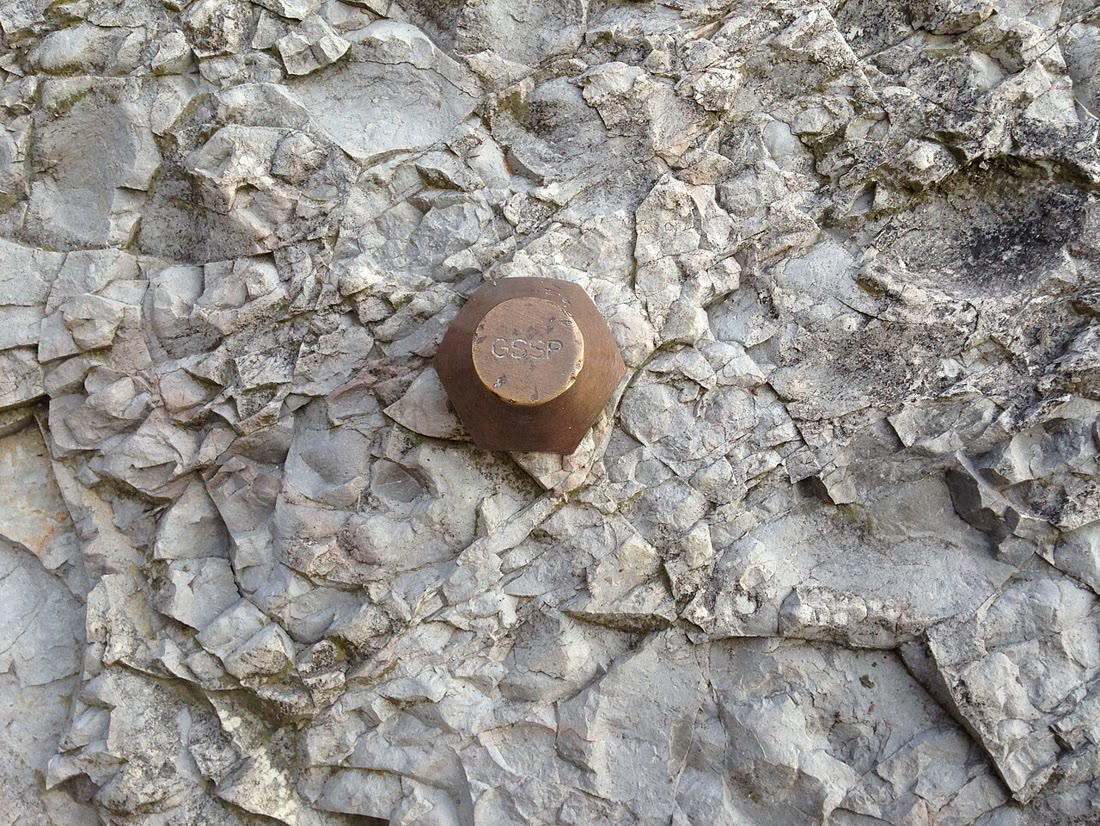
\includegraphics[width=0.62\linewidth]{images/book3/b1-golden-spike-zumaia.jpg}

{\small Le clou d'or de l'\omterm{def:b1:stratigraphic-scale:chronostratigraphy}{étage} Sélandien dans la coupe de Zumaia~: un
repère de bronze frappé GSSP, scellé au sommet du banc de calcaire le plus haut d'une
\omterm{def:b1:stratigraphic-scale:lithostratigraphy}{formation}, à la base des marnes rouges de la suivante. (Josugoni,
CC~BY-SA~4.0, via Wikimedia Commons.)}
\label{fig:b1:stratigraphic-scale:zumaia}
\end{omfigure}
% ledger: commons:zumaia-gssp, gssp:selandian

\begin{recall}
Dans un empilement de couches qui n'a pas été retourné, chaque couche est plus jeune que
celle qui est en dessous~; une structure qui recoupe des roches est plus jeune qu'elles~;
les fossiles changent des couches plus anciennes aux plus jeunes dans le même ordre partout~;
l'histoire de la Terre est divisée en ères et en périodes géologiques, chacune avec un
âge en années pour son début, rassemblées dans une charte internationale (livre~1,
année~7). Un log de forage enregistre les unités rencontrées en fonction de la profondeur, et la \omterm{def:b1:cross-sections:log}{corrélation}
apparie les mêmes unités d'un log à l'autre (\cref{def:b1:cross-sections:log})~; une
\omterm{def:b1:cross-sections:unconformity}{discordance} est une surface d'érosion ou de non-dépôt
(\cref{def:b1:cross-sections:unconformity}). Un \omterm{def:b1:clastic-sediments:facies}{faciès sédimentaire} est un corps de
roche dont les caractères enregistrent son \omterm{def:b1:clastic-sediments:facies}{milieu de dépôt}
(\cref{def:b1:clastic-sediments:facies}). Les volumes de biologie décrivent comment
les espèces apparaissent et s'éteignent, et les quelques extinctions de masse où une grande
part de toutes les espèces a disparu en peu de temps.
\end{recall}

\section{Trois façons de diviser les roches}\label{sec:b1:stratigraphic-scale:three}

Un géologue qui décrit une falaise peut diviser le même empilement de bancs de trois façons~: selon
ce dont les roches sont faites, selon les fossiles qu'elles contiennent, et selon le temps pendant
lequel elles se sont déposées. Les trois divisions répondent à des questions différentes, et
leurs limites n'ont pas à coïncider. Les règles de dénomination et de définition de chaque sorte
d'unité sont fixées par accord international.
% ledger: isg:lithostratigraphy

\begin{definition}[Formation, membre, groupe]\label{def:b1:stratigraphic-scale:lithostratigraphy}
Une \emph{unité lithostratigraphique}\index{unite lithostratigraphique@unité lithostratigraphique} est un corps de
roche défini et reconnu par sa lithologie et sa position parmi d'autres
corps, quel que soit son âge. L'unité de base est la
\emph{formation}\index{formation (lithostratigraphique)}~: un corps de roche assez distinct
de ses voisins pour être cartographié à l'échelle de la région, et en lequel
toute la colonne doit se diviser. Un \emph{membre}\index{membre (lithostratigraphique)} est une
subdivision nommée d'une formation, distinguée par sa
lithologie~; un \emph{groupe}\index{groupe (lithostratigraphique)} est une succession de
deux formations ou plus ayant en commun des caractères lithologiques significatifs. Un
nom formel associe un nom géographique local au rang ou à la roche dominante~:
le grès de Kell, la formation des argilites de Mardon.
\end{definition}
% ledger: isg:lithostratigraphy

Une \omterm{def:b1:stratigraphic-scale:lithostratigraphy}{formation} peut avoir moins d'un mètre d'épaisseur ou plusieurs milliers de mètres. On ne
l'étend loin de sa coupe type que dans la mesure où sa lithologie peut être
reconnue, si bien que ses limites suivent la roche, non le temps.
% ledger: isg:lithostratigraphy

\begin{definition}[Biozone, fossile stratigraphique, première apparition]\label{def:b1:stratigraphic-scale:biozone}
Une \emph{biozone}\index{biozone} est un corps de strates défini ou caractérisé par
les fossiles qu'il contient. Une \emph{biozone d'extension}\index{biozone d'extension} contient les occurrences connues d'un seul
taxon~; une \emph{biozone d'intervalle}\index{biozone d'intervalle} est le corps de strates compris entre deux
horizons fossilifères spécifiés, par exemple les premières occurrences de deux taxons. La
\emph{première apparition}\index{premiere apparition@première apparition} (FAD) d'un taxon est
l'horizon de sa première occurrence, la \emph{dernière
apparition}\index{derniere apparition@dernière apparition} celui de
sa dernière. Un \emph{fossile stratigraphique}\index{fossile stratigraphique} est un taxon servant à
reconnaître une biozone~: les meilleurs sont largement répandus, abondants, faciles à identifier et
de courte durée de vie.
\end{definition}
% ledger: isg:biostratigraphy, og:stratigraphy-principles

Un horizon fossilifère n'a pas d'épaisseur~; une \omterm{def:b1:stratigraphic-scale:biozone}{biozone} peut faire quelques mètres ou quelques centaines de mètres
d'épaisseur selon la vitesse à laquelle le sédiment s'est accumulé pendant que vivaient les taxons.
Comme les espèces évoluent et ne réapparaissent jamais une fois éteintes, l'assemblage de chaque
âge est unique. Certains des meilleurs \omterm{def:b1:stratigraphic-scale:biozone}{fossiles stratigraphiques} sont des microfossiles, tels que
les foraminifères et les conodontes~: répandus, abondants, et assez petits pour être
récupérés dans les déblais d'un forage.
% ledger: isg:biostratigraphy, og:stratigraphy-principles

\begin{definition}[Unités chronostratigraphiques et géochronologiques]\label{def:b1:stratigraphic-scale:chronostratigraphy}
Une \emph{unité chronostratigraphique}\index{unite chronostratigraphique@unité chronostratigraphique} est le corps de
toutes les roches formées pendant un intervalle donné du temps géologique, et seulement pendant
celui-ci~; ses limites sont des surfaces de même âge. L'intervalle de temps lui-même est une
\emph{unité géochronologique}\index{unite geochronologique@unité géochronologique}. Les rangs, du
plus petit, sont l'\emph{étage}\index{etage (chronostratigraphique)@étage (chronostratigraphique)} (son temps~:
un âge), la \emph{série}\index{serie (chronostratigraphique)@série (chronostratigraphique)} (une époque), le
\emph{système}\index{systeme (chronostratigraphique)@système (chronostratigraphique)} (une période), l'érathème (une
ère) et l'éonothème (un éon)~; chaque unité est faite de plusieurs unités consécutives du
rang inférieur.
\end{definition}
% ledger: isg:chronostratigraphy

Les deux mots décrivent la même division vue comme roche ou comme temps
(\cref{tab:b1:stratigraphic-scale:ranks})~: les roches du \omterm{def:b1:stratigraphic-scale:chronostratigraphy}{Système} jurassique se sont
déposées pendant la Période jurassique, et la \omterm{def:b1:stratigraphic-scale:chronostratigraphy}{Série} du Jurassique inférieur pendant
l'Époque du Jurassique précoce. L'\omterm{def:b1:stratigraphic-scale:chronostratigraphy}{étage} est la plus petite unité reconnue dans le monde
entier.
% ledger: isg:chronostratigraphy, chart:danian

\begin{table}[htbp]
\centering
\begin{tabular}{lll}
\hline
chronostratigraphique (roche) & \omterm{def:b1:stratigraphic-scale:chronostratigraphy}{unité géochronologique} (temps) & exemple \\
\hline
éonothème & éon     & Phanérozoïque \\
érathème  & ère     & Cénozoïque \\
\omterm{def:b1:stratigraphic-scale:chronostratigraphy}{système}   & période & Paléogène \\
\omterm{def:b1:stratigraphic-scale:chronostratigraphy}{série}     & époque  & Paléocène \\
\omterm{def:b1:stratigraphic-scale:chronostratigraphy}{étage}     & âge     & Danien (\qtyrange{66.00}{61.66}{\Ma}) \\
\hline
\end{tabular}
\caption{Les rangs des \omterm{def:b1:stratigraphic-scale:chronostratigraphy}{unités chronostratigraphiques} et géochronologiques, avec les
unités qui contiennent le Danien, premier \omterm{def:b1:stratigraphic-scale:chronostratigraphy}{étage} du Cénozoïque.}
\label{tab:b1:stratigraphic-scale:ranks}
\end{table}
% ledger: isg:chronostratigraphy, chart:danian

\section{Les principes et la corrélation}\label{sec:b1:stratigraphic-scale:principles}

Avant qu'aucune roche puisse être datée en années, l'ordre des événements était lu dans les
roches elles-mêmes. Les principes de base de la stratigraphie furent énoncés en 1669 par
Nicolas Steno~; entre 1785 et 1800 Hutton et William Smith y ajoutèrent l'emploi
des couches comme intervalles de temps et de leurs fossiles pour les reconnaître.
% ledger: og:stratigraphy-principles, usgs:hutton-smith

\begin{definition}[Principes de la stratigraphie]\label{def:b1:stratigraphic-scale:principles}
\begin{enumerate}
  \item Le \emph{principe de superposition}\index{principe de superposition}~: dans une suite de couches sédimentaires qui n'a pas été renversée,
        chaque couche est plus jeune que celle sur laquelle elle repose.
  \item Le \emph{principe d'horizontalité originelle}\index{principe d'horizontalite originelle@principe d'horizontalité originelle}~: les sédiments et les coulées de lave se déposent
        horizontalement, ou presque --- légèrement inclinés au bord d'un
        bassin.
  \item Le \emph{principe de continuité latérale}\index{principe de continuite laterale@principe de continuité latérale}~: dans un bassin, une couche s'étend sans interruption dans toutes les
        directions jusqu'à s'amincir au bord du bassin ou contre un
        obstacle~; une couche coupée par une vallée se poursuit de l'autre côté.
  \item Le \emph{principe de recoupement}\index{principe de recoupement}~: un corps ou une structure qui recoupe des
        roches --- un dyke, une faille, une surface d'érosion --- est plus jeune que les
        roches qu'il coupe.
  \item Le \emph{principe de succession faunique}\index{principe de succession faunique}~: les taxons fossiles se succèdent dans le même ordre dans
        toutes les régions, si bien que les roches contenant le même assemblage sont du même
        âge.
\end{enumerate}
\end{definition}
% ledger: og:stratigraphy-principles, eli:relative-dating, usgs:fossil-succession, isg:chronostratigraphy

Les principes ne sont pas d'égale force. La superposition donne un ordre que toute
autre méthode doit respecter. L'horizontalité originelle est ce qui fait d'un banc incliné un
témoin d'une déformation ultérieure. La continuité latérale est ce qui permet à un géologue de
tracer la même couche des deux côtés d'une vallée et, sur une distance limitée, un
plan de stratification suivi sur le terrain est la meilleure ligne de même âge qui existe.
La succession faunique est celle qui traverse les océans~; elle fait l'objet des
paragraphes suivants.
% ledger: isg:chronostratigraphy, og:stratigraphy-principles

\subsection*{La corrélation par biozones}

La \omterm{def:b1:cross-sections:log}{corrélation} par les fossiles compare l'ordre des premières et \omterm{def:b1:stratigraphic-scale:biozone}{dernières apparitions} dans deux
coupes (figure ci-dessous). Les deux ne sont pas également fiables. Le plus haut fossile
d'un taxon trouvé dans une coupe dépend du nombre de ceux qui ont été préservés~: là où ils sont
rares, le dernier trouvé peut se situer bien en dessous du niveau auquel le taxon a réellement
disparu, et un fossile érodé et redéposé peut apparaître au-dessus. Une \omterm{def:b1:stratigraphic-scale:biozone}{première
apparition} peut aussi être déplacée, mais un taxon répandu qui s'est propagé rapidement est
atteint à peu près au même niveau dans tout un bassin.
% ledger: isg:biostratigraphy

\begin{omfigure}
\begin{tikzpicture}[font=\footnotesize, y=0.13cm]
  % section 1: 40 m, sandstone 0-14, shale 14-40
  \fill[lith sandstone] (0,0) rectangle (0.8,14);
  \fill[lith shale] (0,14) rectangle (0.8,40);
  \draw[black!70] (0,0) rectangle (0.8,40);
  \node[anchor=south, font=\small] at (1.4,41.5) {coupe 1};
  \foreach \x/\a/\b/\t in {1.1/0/27/a, 1.4/10/34/b, 1.7/20/40/c, 2.0/30/40/d} {
    \draw[line width=2.2pt, omThm] (\x,\a) -- (\x,\b);
    \node[anchor=base, font=\scriptsize] at (\x,-4.5) {\t};
  }
  \foreach \y/\z in {5/a, 15/b, 25/c, 35/d}
    \node[anchor=east, font=\scriptsize] at (-0.1,\y) {zone \z};
  \foreach \y in {10,20,30} \draw[black!50] (-1.3,\y) -- (0,\y);
  % scale bar
  \draw[thick] (-1.5,0) -- (-1.5,10) node[midway, anchor=east, font=\scriptsize] {\qty{10}{m}};
  % section 2: 24 m, sandstone 0-3, shale 3-24
  \begin{scope}[xshift=7cm]
    \fill[lith sandstone] (0,0) rectangle (0.8,3);
    \fill[lith shale] (0,3) rectangle (0.8,24);
    \draw[black!70] (0,0) rectangle (0.8,24);
    \node[anchor=south, font=\small] at (1.4,25.5) {coupe 2};
    \foreach \x/\a/\b/\t in {1.1/0/13/a, 1.4/6/20/b, 1.7/12/24/c, 2.0/18/24/d} {
      \draw[line width=2.2pt, omThm] (\x,\a) -- (\x,\b);
      \node[anchor=base, font=\scriptsize] at (\x,-4.5) {\t};
    }
    \foreach \y/\z in {3/a, 9/b, 15/c, 21/d}
      \node[anchor=west, font=\scriptsize] at (2.3,\y) {zone \z};
    \foreach \y in {6,12,18} \draw[black!50] (0.8,\y) -- (2.3,\y);
  \end{scope}
  % correlation of the first appearances
  \foreach \u/\v/\t in {10/6/b, 20/12/c, 30/18/d}
    \draw[densely dashed, omThm!70!black] (2.15,\u) -- (6.85,\v)
      node[pos=0.5, fill=white, inner sep=1pt, font=\scriptsize] {FAD \t};
\end{tikzpicture}

{\small Un tableau d'extension et une \omterm{def:b1:cross-sections:log}{corrélation} par \omterm{def:b1:stratigraphic-scale:biozone}{biozones} (taxons inventés \emph{a} à
\emph{d}). Les barres épaisses sont les extensions des taxons dans chaque coupe. Trois
\omterm{def:b1:stratigraphic-scale:biozone}{biozones d'intervalle} sont limitées par les \omterm{def:b1:stratigraphic-scale:biozone}{premières apparitions} de \emph{b}, \emph{c} et
\emph{d}, qui sont reliées d'une coupe à l'autre (tirets). La \omterm{def:b1:stratigraphic-scale:biozone}{dernière
apparition} de \emph{a} tombe dans la partie haute de la zone~\emph{c} dans la coupe~1
et près de sa base dans la coupe~2~: c'est un moins bon guide. Les zones sont plus minces dans
la coupe~2, où le sédiment s'est accumulé plus lentement.}
\label{fig:b1:stratigraphic-scale:range-chart}
\end{omfigure}

\begin{method}[Corréler des coupes par biozones]\label{met:b1:stratigraphic-scale:biozones}
\begin{enumerate}
  \item Porter, pour chaque coupe, l'extension de chaque taxon en fonction de la hauteur~: de
        sa première à sa dernière occurrence.
  \item Choisir les horizons fossilifères qui définissent les zones --- de préférence des \omterm{def:b1:stratigraphic-scale:biozone}{premières
        apparitions} de taxons répandus et indépendants du faciès.
  \item Tracer les limites de zones dans chaque coupe à ces horizons.
  \item Relier les mêmes horizons d'une coupe à l'autre~; vérifier que les lignes
        ne se croisent pas, comme l'exige la superposition.
  \item Lire, entre deux lignes, l'épaisseur de chaque zone dans chaque coupe~;
        là où une zone manque, chercher une \omterm{def:b1:cross-sections:unconformity}{discordance} ou un changement de
        faciès avant de conclure que le taxon est absent.
\end{enumerate}
\end{method}

Une \omterm{def:b1:stratigraphic-scale:biozone}{biozone} ne vaut que par l'indépendance de ses fossiles vis-à-vis du
milieu. Un bivalve qui ne vivait que sur des rivages sableux ne se trouve que dans des
grès~; le suivre d'une coupe à l'autre revient à suivre le grès, non le
temps. La \omterm{def:b1:cross-sections:log}{corrélation} biostratigraphique n'est donc pas nécessairement une \omterm{def:b1:cross-sections:log}{corrélation}
du temps~: elle peut suivre un faciès dont l'âge change d'un lieu à l'autre.
% ledger: isg:biostratigraphy

\subsection*{Les limites qui traversent le temps}

Des sédiments différents se déposent en même temps en des lieux différents~: du sable sur
le rivage, de la boue au large, du calcaire plus loin sur une plate-forme privée de sable. Une ligne de
même âge passe donc d'une lithologie à une autre. Inversement, une
limite lithologique tracée à travers un bassin n'a pas à être une ligne de même âge
du tout.
% ledger: og:stratigraphy-principles, isg:chronostratigraphy

\begin{definition}[Limite diachrone]\label{def:b1:stratigraphic-scale:diachronous}
Une limite est \emph{diachrone}\index{limite diachrone} quand son âge
change d'un lieu à l'autre le long d'elle. Les limites de \omterm{def:b1:stratigraphic-scale:lithostratigraphy}{formations} et de
faciès sont couramment diachrones~; les limites d'\omterm{def:b1:stratigraphic-scale:chronostratigraphy}{unités chronostratigraphiques}
ne le sont pas, par définition.
\end{definition}
% ledger: isg:lithostratigraphy, isg:chronostratigraphy, isg:biostratigraphy

Le cas classique est une transgression~: le \omterm{def:b1:diagenesis-basins:eustasy}{niveau marin relatif} monte plus vite que le
sédiment ne peut combler la place faite, et le rivage se déplace vers l'intérieur des terres. Le sable de plage
se dépose au rivage à chaque instant, si bien qu'une nappe de grès s'étend
vers l'intérieur avec lui~; la boue du large suit par-dessus. Le sommet du grès est
alors la trace du rivage mobile~: jeune vers l'intérieur, vieux vers le large
(figure ci-dessous). L'ordre des faciès vu dans une seule coupe verticale --- grès
sous argilite sous calcaire --- répète leur ordre sur la plate-forme à un seul
instant~; le volume de troisième année en fait la base de ses modèles de faciès.
% ledger: og:stratigraphy-principles, isg:lithostratigraphy

\begin{omfigure}
\begin{tikzpicture}[font=\footnotesize, x=1cm, y=1cm]
  % basement surface B(x) = 1.6 (1 - x/14), rising towards the land on the left
  \fill[lith granite] (0,-0.5) -- (0,1.6) -- (14,0) -- (14,-0.5) -- cycle;
  \fill[lith sandstone] (0,1.6) -- (14,0) -- (14,0.5) -- (0,2.1) -- cycle;
  \fill[lith shale] (0,2.1) -- (14,0.5) -- (14,1.5) -- (0,3.1) -- cycle;
  \fill[lith limestone] (0,3.1) -- (14,1.5) -- (14,3.6) -- (0,3.6) -- cycle;
  \draw[unconformity] (0,1.6) -- (14,0);
  \draw[black!70] (0,2.1) -- (14,0.5) (0,3.1) -- (14,1.5);
  \draw[black!70] (0,-0.5) rectangle (14,3.6);
  % time lines: horizontal, from the basement (or the left edge) to the right edge
  \foreach \y/\t in {0.6/1, 1.1/2, 1.6/3, 2.1/4, 2.6/5, 3.1/6} {
    \pgfmathsetmacro{\xs}{max(0, 14*(1-\y/1.6))}
    \draw[omThm, thick, densely dashed] (\xs,\y) -- (14,\y) node[anchor=west, text=black] {$t_\t$};
  }
  % two sections
  \foreach \x/\n in {3/1, 11/2} {
    \draw[very thick, black] (\x,-0.5) -- (\x,3.6);
    \node[anchor=south, font=\small] at (\x,3.65) {coupe \n};
  }
  \node[fill=white, inner sep=1pt, font=\scriptsize] at (5.6,1.21) {grès};
  \node[fill=white, inner sep=1pt] at (12.6,1.2) {argilite};
  \node[fill=white, inner sep=1pt] at (7.0,3.25) {calcaire};
  \node[fill=white, inner sep=1pt] at (12.0,-0.25) {socle};
  \draw[-{Stealth}, thick] (5.6,4.35) -- (3.6,4.35) node[anchor=east] {terre};
  \draw[-{Stealth}, thick] (8.4,4.35) -- (10.4,4.35) node[anchor=west] {mer};
\end{tikzpicture}

{\small Une nappe de grès déposée pendant une transgression (schématique, échelle verticale
exagérée). Les lignes en tirets $t_1$ à $t_6$ joignent des points de même âge,
$t_1$ le plus ancien. Là où l'une rejoint le socle, elle commence au rivage de
son époque~; vers le large elle passe du sable à la boue et, dans les plus jeunes, au calcaire.
Le sommet du grès
se situe entre $t_1$ et $t_2$ dans la coupe~2 mais entre $t_3$ et $t_4$ dans la
coupe~1~: la limite de \omterm{def:b1:stratigraphic-scale:lithostratigraphy}{formation} est \omterm{def:b1:stratigraphic-scale:diachronous}{diachrone}, plus jeune vers la terre.}
\label{fig:b1:stratigraphic-scale:diachronous}
\end{omfigure}

À quelle vitesse l'âge de la limite change-t-il le long d'elle~? Sur une plaine côtière qui s'élève
doucement vers l'intérieur, la réponse relève de la géométrie.

\begin{proposition}[Vitesse d'une transgression]\label{prop:b1:stratigraphic-scale:transgression}
Une plaine côtière s'élève vers l'intérieur avec la pente uniforme $s$, et le \omterm{def:b1:diagenesis-basins:eustasy}{niveau
marin relatif} monte au rythme constant $R$, sans apport de sédiment au rivage. Le
rivage se déplace alors vers l'intérieur à la vitesse
\[
  u = \frac{R}{s},
\]
et une limite qui suit le rivage est plus jeune, en un point à une distance $d$
plus loin à l'intérieur, de $\Delta t = d/u = d\,s/R$.
\end{proposition}

\begin{proof}
Prenons $x$ comme distance vers l'intérieur depuis un point fixe et $z$ comme hauteur~; la
plaine est la droite $z = s x$, et la surface de la mer à l'instant $t$ est
$z = z_0 + R t$. Le rivage est là où elles se rencontrent~: $s\,x(t) = z_0 + R t$, donc
$x(t) = (z_0 + R t)/s$ et $\mathrm dx/\mathrm dt = R/s$. Le rivage atteint
un point situé à la distance $d$ plus loin à l'intérieur après le temps $d/u = d\,s/R$.
\end{proof}

Le rapport est grand parce que les plaines côtières sont presque plates. Une montée de
\qty{10}{m} par million d'années sur une plaine de pente $1$ pour $2000$ fait avancer le rivage
de \qty{20}{km} vers l'intérieur par million d'années~; un sommet de grès qui ressemble à une seule
surface dans une falaise est alors plus jeune d'un million d'années à \qty{20}{km} à l'intérieur. Le sédiment
apporté au rivage ralentit la transgression ou l'inverse.

\subsection*{Les lignes de même âge}

Qu'est-ce qui corrèle le temps, alors, si la lithologie ne le fait pas et les fossiles seulement
approximativement~? Les meilleures lignes sont faites par des événements qui laissent une trace partout
à la fois. Une cendre volcanique tombe sur une vaste aire en ce qui est, géologiquement, un
instant, et se dépose sur le sable, la boue et le calcaire sans distinction~: un banc de cendre est une ligne de même
âge qui traverse les limites de faciès, et il peut souvent être daté en années par les
méthodes du \cref{ch:b1:radiometric-methods}. Les inversions du champ magnétique
terrestre, traitées dans le volume de troisième année, sont enregistrées dans des roches de nombreuses sortes et peuvent
être reconnues dans le monde entier une fois leur ordre connu~; de même les brusques variations des
isotopes du carbone, telles que celle qui marque la base de l'Yprésien
(\cref{tab:b1:stratigraphic-scale:gssps}). Entre deux
niveaux datés, l'âge d'un banc quelconque s'estime en supposant que le sédiment
s'est accumulé à vitesse constante.
% ledger: isg:chronostratigraphy

\begin{proposition}[Âge entre deux niveaux datés]\label{prop:b1:stratigraphic-scale:interpolation}
Deux bancs aux hauteurs $z_1 < z_2$ d'une coupe continue ont les âges
$t_1 > t_2$. Si le sédiment s'est accumulé à vitesse constante entre eux, un
niveau à la hauteur $z$ entre eux a l'âge
\[
  t = t_1 - f\,(t_1 - t_2), \qquad f = \frac{z - z_1}{z_2 - z_1},
\]
et la vitesse d'accumulation est $r = (z_2 - z_1)/(t_1 - t_2)$. Si les deux âges
ont pour incertitudes-types indépendantes $\sigma_1$ et $\sigma_2$, l'âge
interpolé a pour incertitude
\[
  \sigma_t = \sqrt{(1 - f)^2 \sigma_1^2 + f^2 \sigma_2^2}.
\]
\end{proposition}

\begin{proof}
À vitesse constante $r$, la hauteur croît linéairement avec le temps~: $z - z_1 = r\,(t_1
- t)$, puisque les âges décroissent vers le haut. En $z_2$, $z_2 - z_1 = r\,(t_1 - t_2)$, ce qui
donne $r$~; en divisant les deux relations on obtient $t_1 - t = f\,(t_1 - t_2)$. L'âge
est la combinaison linéaire $t = (1 - f)\,t_1 + f\,t_2$ de deux grandeurs
indépendantes~; la variance de $a X + b Y$ pour $X$ et $Y$ indépendantes est $a^2
\operatorname{Var} X + b^2 \operatorname{Var} Y$, ce qui donne $\sigma_t$.
\end{proof}

L'incertitude est la plus petite entre les deux bancs datés et n'y dépasse jamais
la plus grande de $\sigma_1$ et $\sigma_2$. La vraie limite est l'hypothèse~:
le sédiment s'accumule par à-coups, peut s'arrêter lors de lacunes cachées, et se compacte
différemment dans le sable et dans la boue (\cref{prop:b1:diagenesis-basins:solid}), si bien que
l'âge interpolé n'est pas meilleur que la régularité de la coupe.

\section{Les stratotypes de limite}\label{sec:b1:stratigraphic-scale:gssp}

Une \omterm{def:b1:stratigraphic-scale:chronostratigraphy}{unité chronostratigraphique} est définie dans la roche avant d'être datée. L'ancienne
pratique décrivait chaque \omterm{def:b1:stratigraphic-scale:chronostratigraphy}{étage} par une coupe type de l'unité entière~; mais le sommet
d'une coupe type et la base de la suivante, choisis en des lieux différents, pouvaient
laisser entre eux une lacune de temps non attribué ou un chevauchement. La pratique moderne
ne définit que la limite inférieure de chaque unité en un point d'une coupe~; la
limite supérieure est la limite inférieure de l'unité suivante. Aucun intervalle de temps ne peut
alors tomber entre deux unités ni appartenir aux deux.
% ledger: isg:stratotype, isg:chronostratigraphy

\begin{definition}[Stratotype de limite, stratotype d'unité, GSSP]\label{def:b1:stratigraphic-scale:gssp}
Un \emph{stratotype}\index{stratotype} est la coupe de roche désignée qui
sert de référence standard à une unité ou à une limite. Un \emph{stratotype
d'unité}\index{stratotype d'unite@stratotype d'unité} est la coupe type d'une unité entière~; un
\emph{stratotype de limite}\index{stratotype de limite} est la coupe qui
contient le point spécifique définissant une limite entre deux unités. Un
\emph{stratotype limite mondial (section et point)}\index{stratotype limite mondial (GSSP)} (GSSP) est le stratotype de limite d'une
unité de l'échelle chronostratigraphique internationale~: un point unique dans une unique
coupe, choisi par accord international, qui définit la base d'un \omterm{def:b1:stratigraphic-scale:chronostratigraphy}{étage}
et de toute unité plus grande qui commence avec lui.
\end{definition}
% ledger: isg:stratotype, isg:chronostratigraphy, gssp:protocol

Le GSSP est un point dans la roche, non un âge. Son âge en années est ce que donne la meilleure
datation de ce point, et il peut être affiné sans que le point bouge. La
coupe est choisie pour que le point puisse être retrouvé ailleurs~: dépôt continu
à travers la limite (jamais à une \omterm{def:b1:cross-sections:unconformity}{discordance}, où le temps manquant rendrait
la limite ambiguë), de préférence marin, riche en fossiles bien préservés de taxons
répandus, sans changement de faciès à ce niveau, peu déformé ou
altéré, accessible et protégé. Surtout, le point est placé à un niveau
qui coïncide avec un signal choisi --- le plus souvent la \omterm{def:b1:stratigraphic-scale:biozone}{première apparition} d'un
taxon --- au sein d'un intervalle riche en d'autres signaux (bancs de cendre, inversions
magnétiques, variations isotopiques) par lesquels le niveau peut être reconnu au loin. Un
repère permanent, le clou d'or, est placé au point.
% ledger: isg:chronostratigraphy, isg:stratotype, gssp:protocol

\begin{inthefield}[Comment une limite est choisie]
Une limite est étudiée par un groupe de travail de la sous-commission chargée du
\omterm{def:b1:stratigraphic-scale:chronostratigraphy}{système}, qui compare des coupes candidates, les décrit banc par banc, échantillonne leurs
fossiles, bancs de cendre et isotopes, et rédige une proposition. Une proposition exige une
supermajorité --- plus de \qty{60}{\%} --- des membres votants de la
sous-commission, une vingtaine de spécialistes~; elle passe ensuite aux membres votants de la
Commission internationale de stratigraphie, les dirigeants et les
présidents de ses dix-sept sous-commissions, et enfin au comité exécutif de
l'Union internationale des sciences géologiques, dont l'approbation la ratifie. Les
résultats sont publiés, le repère est scellé dans la roche, et aucune modification d'une limite
nouvellement établie ne peut être proposée avant dix ans.
\end{inthefield}
% ledger: gssp:protocol

\begin{table}[htbp]
\centering
\small
\begin{tabular}{>{\raggedright\arraybackslash}p{2.4cm}>{\raggedright\arraybackslash}p{1.2cm}>{\raggedright\arraybackslash}p{3.7cm}>{\raggedright\arraybackslash}p{5.6cm}c}
\hline
base de & âge (\unit{\Ma}) & coupe & repère du point & ratifié \\
\hline
Fortunien (Cambrien) & 538.8 & Fortune Head, Terre-Neuve, Canada & \omterm{def:b1:stratigraphic-scale:biozone}{première apparition} du fossile de trace \emph{Trichophycus pedum} & 1992 \\
Lochkovien (Dévonien) & 419.62 & Klonk, près de Prague, République tchèque & \omterm{def:b1:stratigraphic-scale:biozone}{première apparition} du graptolite \emph{Monograptus uniformis} & 1972 \\
Indusien (Trias) & 251.902 & Meishan, Zhejiang, Chine & \omterm{def:b1:stratigraphic-scale:biozone}{première apparition} du conodonte \emph{Hindeodus parvus}, base du banc~27c & 2001 \\
Danien (Paléogène) & 66.00 & Oued Djerfane, El Kef, Tunisie & base d'une argile de limite sombre de \qty{50}{cm}~; anomalie en iridium & 1991 \\
Sélandien & 61.66 & Zumaia, Espagne & base des marnes rouges~; seconde radiation d'un \omterm{def:b1:stratigraphic-scale:lithostratigraphy}{groupe} de nannofossiles & 2008 \\
Yprésien (Éocène) & 56.00 & Dababiya, près de Louxor, Égypte & base d'une excursion des isotopes du carbone & 2003 \\
Chibanien & 0.774 & Chiba, Japon & base d'une téphra, juste sous une inversion magnétique & 2020 \\
Meghalayen & 0.0042 & grotte de Mawmluh, Meghalaya, Inde & un niveau situé à \qty{7.45}{mm} de profondeur dans un spéléothème & 2018 \\
\hline
\end{tabular}
\caption{Huit GSSP. Les repères sont des \omterm{def:b1:stratigraphic-scale:biozone}{premières apparitions} de taxons, une
anomalie géochimique, une excursion isotopique, une inversion magnétique et un événement climatique enregistré
dans un dépôt de grotte.}
\label{tab:b1:stratigraphic-scale:gssps}
\end{table}
% ledger: gssp:fortunian, gssp:lochkovian, gssp:induan, gssp:danian, gssp:selandian, gssp:ypresian, gssp:chibanian, gssp:meghalayan

Le \cref{tab:b1:stratigraphic-scale:gssps} montre combien les signaux choisis sont variés.
Les limites du Paléozoïque et du Mésozoïque du tableau reposent sur des \omterm{def:b1:stratigraphic-scale:biozone}{premières apparitions} de
fossiles, un graptolite et un conodonte~; à la base du Cambrien le fossile est un
fossile de trace, la marque laissée dans le sédiment par l'activité d'un animal plutôt que
l'animal lui-même. Dans les exemples du Cénozoïque les signaux sont chimiques et
physiques~: l'iridium du Danien, l'excursion des isotopes du carbone de l'Yprésien,
l'inversion magnétique qui se trouve \qty{1.1}{m} au-dessus du point du Chibanien. La
plus jeune limite du tableau n'est pas du tout dans une roche marine~: la base du
Meghalayen est un niveau à l'intérieur d'un spéléothème, un dépôt formé dans une grotte, qui enregistre
un événement climatique d'il y a 4200 ans.
% ledger: gssp:fortunian, gssp:danian, gssp:ypresian, gssp:chibanian, gssp:meghalayan

\begin{dated}{2026}
% ledger: gssp:count, chart:stage-count
En octobre 2026 le tableau de la Commission internationale de stratigraphie dénombrait
80 GSSP ratifiés, et deux autres proposés. Le premier fut ratifié en 1972, à
Klonk~; le plus récent en 2024, quand deux limites du Silurien, jusque-là
définies au pays de Galles, furent déplacées vers de nouvelles coupes en Espagne et en
République tchèque. Sur les 101 \omterm{def:b1:stratigraphic-scale:chronostratigraphy}{étages} du Phanérozoïque de la charte, 21 n'avaient toujours aucun
GSSP ratifié~; leurs bases sont provisoires.
\end{dated}

Sous le Phanérozoïque, l'échelle est le plus souvent divisée autrement. À l'exception de son
plus jeune \omterm{def:b1:stratigraphic-scale:chronostratigraphy}{système}, l'Édiacarien, le Précambrien est découpé à des âges ronds choisis par
accord --- les divisions sont définies en années, non par des points dans la roche.
% ledger: isg:chronostratigraphy

\section{Les extinctions de masse comme repères}\label{sec:b1:stratigraphic-scale:extinctions}

Les volumes de biologie décrivent les extinctions de masse comme des moments où une grande part des
espèces a disparu en un temps géologiquement court. Pour la stratigraphie, un tel
événement est un cadeau~: un horizon présent sur chaque continent et dans chaque océan,
au travers duquel les assemblages fossiles changent complètement. Deux d'entre eux délimitent les
trois ères du Phanérozoïque.
% ledger: schulte:kpg, burgess:end-permian

\subsection*{La fin du Crétacé}

En 1980, L.~W.~Alvarez, W.~Alvarez, F.~Asaro et H.~V.~Michel mesurèrent l'iridium
--- l'un des métaux du \omterm{def:b1:stratigraphic-scale:lithostratigraphy}{groupe} du platine, appauvri dans la \omterm{def:b1:layered-earth:layers}{croûte} terrestre par rapport à
son abondance dans le cosmos --- dans des calcaires d'eau profonde à travers la limite
entre le Crétacé et le Tertiaire --- aujourd'hui la limite entre le
Crétacé et le Paléogène, la limite K--Pg. Ils le trouvèrent enrichi d'environ 30 fois par rapport au
fond en Italie, de 160 fois au Danemark et de 20 fois en Nouvelle-Zélande,
exactement au niveau des extinctions. Ils proposèrent qu'un \omterm{def:b1:comparative-planetology:small-bodies}{astéroïde}
de $\qty{10}{km}$ de large, à quatre près, avait frappé la Terre et projeté dans l'atmosphère environ
60 fois sa propre masse de roche pulvérisée~; la poussière se serait
répandue dans le monde entier et aurait obscurci le ciel. L'argile de la limite, firent-ils
remarquer, diffère chimiquement de l'argile des calcaires au-dessus et en dessous.
% ledger: alvarez:iridium

Des travaux ultérieurs ont relié la limite à un seul impact, Chicxulub. La datation argon--argon
place cet impact et la limite avec ses extinctions à moins de \num{32000}
ans l'un de l'autre, et une revue des preuves a conclu que l'impact a déclenché
l'extinction, qui est aussi tombée dans le temps d'un grand épanchement de basalte
en Inde. Le GSSP de la base du Danien --- base du Paléogène et de
tout le Cénozoïque --- est placé à la base de l'argile de limite sombre d'El Kef
en Tunisie, à l'anomalie en iridium. La même limite se voit à terre, dans le
Colorado (figure ci-dessous).
% ledger: renne:kpg, schulte:kpg, gssp:danian, commons:kt-tlsp

\begin{omfigure}
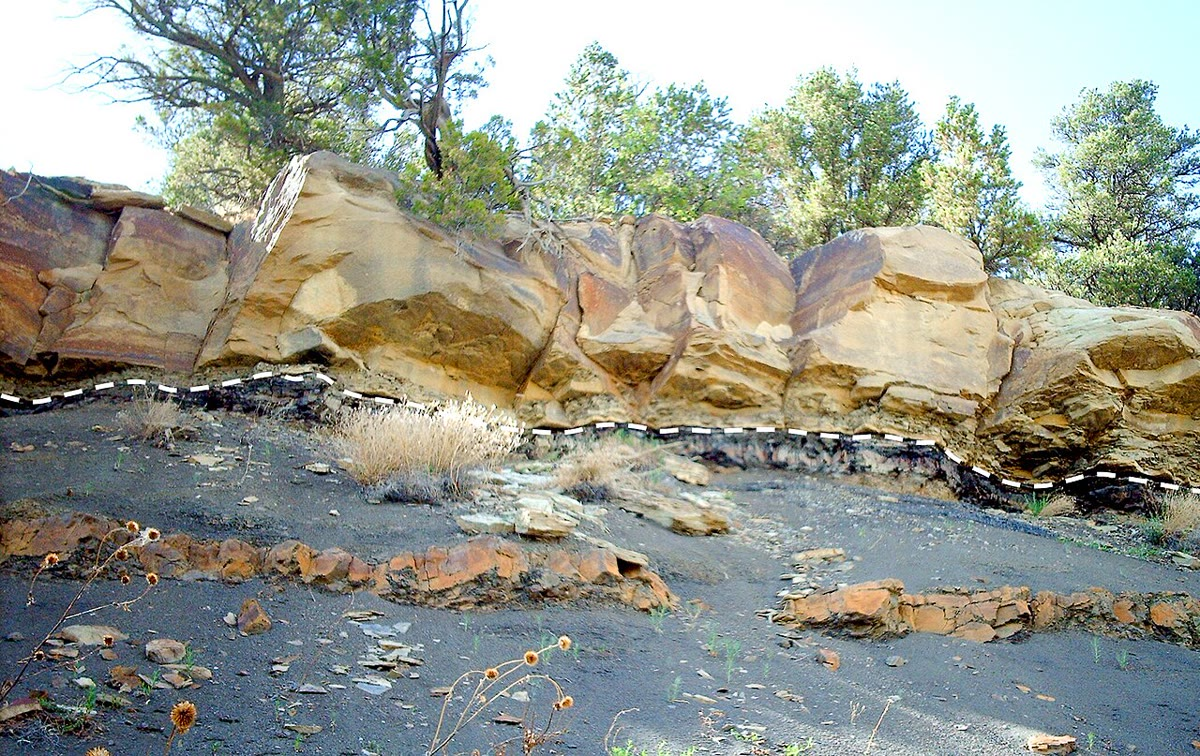
\includegraphics[width=0.78\linewidth]{images/book3/b1-kpg-boundary-trinidad.jpg}

{\small La limite entre le Crétacé et le Paléogène, marquée par la
ligne en tirets, au parc d'État du lac Trinidad, Colorado~: grès au-dessus, bancs sombres
en dessous et le long de la limite. (Nationalparks, CC~BY-SA~2.5,
via Wikimedia Commons~; la ligne en tirets figure sur l'original.)}
\label{fig:b1:stratigraphic-scale:kpg}
\end{omfigure}
% ledger: commons:kt-tlsp

\subsection*{La fin du Permien}

L'extinction de la fin du Permien fut la plus sévère perte de vie marine et
terrestre du dernier demi-milliard d'années. À Meishan en Chine, la coupe qui
contient le GSSP de la base du Trias, cinq bancs de cendre ont été datés par la
méthode uranium--plomb sur zircon. Ils placent l'extinction entre
\qty[uncertainty-mode=separate]{251.941(37)}{\Ma} et \qty[uncertainty-mode=separate]{251.880(31)}{\Ma}~: un intervalle de
\num[uncertainty-mode=separate]{60 \pm 48} milliers d'années. Un net décalage négatif de \qty{3}{\permil} dans
les isotopes du carbone des carbonates la précède, et le cycle du carbone est resté
instable pendant environ \num{500} milliers d'années.
% ledger: burgess:end-permian, gssp:induan

La base du Trias elle-même, \qty[uncertainty-mode=separate]{251.902(24)}{\Ma}, n'est pas placée à
l'extinction mais à la \omterm{def:b1:stratigraphic-scale:biozone}{première apparition} du conodonte \emph{Hindeodus parvus},
un niveau qui tombe dans l'intervalle de l'extinction daté à Meishan. Une
extinction est un ensemble de \omterm{def:b1:stratigraphic-scale:biozone}{dernières apparitions}, que la préservation brouille~; une seule \omterm{def:b1:stratigraphic-scale:biozone}{première
apparition} d'une espèce bien connue fait une ligne plus nette. Les causes des deux extinctions ---
un impact, les grandes provinces basaltiques --- sont l'objet du volume de deuxième année.
% ledger: gssp:induan, isg:biostratigraphy, burgess:end-permian

\section{La charte internationale}\label{sec:b1:stratigraphic-scale:chart}

La charte chronostratigraphique internationale rassemble toutes les unités, des
éonothèmes aux \omterm{def:b1:stratigraphic-scale:chronostratigraphy}{étages}, en un tableau~: leurs noms, la base de chacune en millions
d'années avec son incertitude, une marque pour chaque base définie par un GSSP ratifié,
et une couleur standard pour chaque unité, celle de la Commission de la carte
géologique du monde. La
partie du Phanérozoïque, réduite à ses ères et ses périodes, est dessinée ci-dessous d'après les
valeurs de la charte elle-même.
% ledger: ics:base.Paleozoic, ics:colour.Paleozoic, gssp:count

\begin{omfigure}
\begin{tikzpicture}[font=\footnotesize]
\begin{axis}[y dir=reverse, ymin=0, ymax=538.8, xmin=0, xmax=6.2,
  width=6.6cm, height=11cm, scale only axis, clip=false,
  axis x line=none, axis y line*=left, ytick={0,100,...,500},
  ylabel={âge (\unit{\Ma})}, tick label style={font=\scriptsize}]
  \pgfplotsinvokeforeach{Paleozoic,Mesozoic,Cenozoic,Cambrian,Ordovician,Silurian,Devonian,Carboniferous,Permian,Triassic,Jurassic,Cretaceous,Paleogene,Neogene,Quaternary}{
    \addplot[fill=ics#1, draw=black!70, line width=0.3pt] table[x=x, y=age] {figdata/out/bachelor-1-ics_chart-bar-#1.dat};}
  \addplot[draw=none, nodes near coords, point meta=explicit symbolic,
    every node near coord/.style={anchor=center, rotate=90, font=\scriptsize\bfseries}]
    coordinates {(0.5,395.351) [Paléozoïque] (0.5,158.951) [Mésozoïque] (0.5,33) [Cénozoïque]};
  \addplot[draw=none, nodes near coords, point meta=explicit symbolic,
    every node near coord/.style={anchor=center, font=\scriptsize}]
    coordinates {(2,512.825) [Cambrien] (2,464.975) [Ordovicien] (2,431.36) [Silurien] (2,389.24) [Dévonien] (2,328.88) [Carbonifère] (2,275.401) [Permien] (2,226.651) [Trias] (2,172.25) [Jurassique] (2,104.55) [Crétacé] (2,44.52) [Paléogène] (2,12.81) [Néogène]};
  \addplot[mark=-, mark size=3pt, only marks, nodes near coords, point meta=explicit symbolic,
    every node near coord/.style={anchor=west, xshift=1pt, font=\scriptsize}]
    table[x=x, y=age, meta=lab] {figdata/out/bachelor-1-ics_chart-bases.dat};
  \addplot[only marks, mark=triangle*, mark size=3pt, mark options={rotate=90, fill=omThm, draw=omThm},
    nodes near coords, point meta=explicit symbolic,
    every node near coord/.style={anchor=west, xshift=3pt, font=\scriptsize, text=omThm}]
    coordinates {(4.75,251.902) [fin du Permien] (4.75,66) [fin du Crétacé]};
  \node[anchor=south, font=\scriptsize] at (axis cs:2,0) {Quaternaire};
  \node[anchor=west, font=\scriptsize] at (axis cs:3.0,-14) {0};
  \node[anchor=south, font=\scriptsize\itshape] at (axis cs:0.5,-30) {ère};
  \node[anchor=south, font=\scriptsize\itshape] at (axis cs:2,-30) {période};
  \node[anchor=south, font=\scriptsize\itshape] at (axis cs:3.5,-30) {base (\unit{\Ma})};
\end{axis}
\end{tikzpicture}

{\small Le Phanérozoïque sur la charte internationale~: ses trois ères et douze
périodes, à l'échelle, dans les couleurs de la charte, avec l'âge de la base de chaque
période (incertitudes omises). Les triangles marquent les deux bases qui sont des horizons
d'extinction de masse. Le Quaternaire, long de \qty{2.58}{\Ma}, est la mince bande en
haut.}
\label{fig:b1:stratigraphic-scale:chart}
\end{omfigure}
% computed in figdata/bachelor-1/ics_chart.py; ledger: ics:base.Cambrian, ics:colour.Cambrian (every ics base and colour row of the eras and periods), burgess:end-permian, alvarez:iridium

Les périodes sont très inégales (figure ci-dessus). Le Crétacé a duré
\qty{77.1}{\Ma}, le Néogène \qty{20.46}{\Ma} et le Quaternaire seulement
\qty{2.58}{\Ma}~; la moyenne des douze est de \qty{44.9}{\Ma}. L'inégalité est
héritée~: les \omterm{def:b1:stratigraphic-scale:chronostratigraphy}{systèmes} furent nommés dans des classifications anciennes, avant qu'aucune roche fût
datée en années --- certains noms donnent une position (Paléogène, Néogène, Quaternaire),
certains une roche (Carbonifère, Crétacé), certains un peuple ou un lieu (Ordovicien,
Silurien, Dévonien, Permien) --- et la charte garde les noms tout en définissant
leurs bases par des GSSP. Les âges en années proviennent de la datation isotopique de
roches volcaniques proches des limites, comme les bancs de cendre de Meishan
(\cref{ch:b1:radiometric-methods}), interpolés comme dans la
\cref{prop:b1:stratigraphic-scale:interpolation}~; une nouvelle version de la charte peut
décaler un âge tandis que le GSSP reste où il est.
% ledger: ics:base.Cretaceous, ics:base.Neogene, ics:base.Quaternary, isg:chronostratigraphy, burgess:end-permian

\begin{dated}{2024}
% ledger: iugs:anthropocene
L'Anthropocène, nom proposé en 2001 pour un nouvel intervalle marqué par l'activité
humaine, a été étudié à partir de 2009 par un groupe de travail de la sous-commission de
stratigraphie du Quaternaire. Fin 2023 le groupe a proposé une \omterm{def:b1:stratigraphic-scale:chronostratigraphy}{série} commençant
vers 1950, avec son GSSP dans le sédiment du lac Crawford, en Ontario. Le
vote de la sous-commission, clos le 4 mars 2024, l'a rejetée~: 4 voix pour, 12
contre, 3 abstentions, 3 membres ne votant pas. Les membres votants de la
Commission internationale de stratigraphie ont reconnu le vote. L'Anthropocène
n'est pas une unité de la charte~; il reste un terme informel, largement employé.
\end{dated}

\section{Exercices}

\begin{exercise}[$\star$]\label{exo:b1:stratigraphic-scale:1}
Dire si chaque nom est celui d'une \omterm{def:b1:stratigraphic-scale:lithostratigraphy}{unité lithostratigraphique}, biostratigraphique,
chronostratigraphique ou géochronologique, et donner son rang quand elle en a
un~: (a)~le \omterm{def:b1:stratigraphic-scale:chronostratigraphy}{Système} jurassique~; (b)~la \omterm{def:b1:stratigraphic-scale:lithostratigraphy}{formation} des argilites de Mardon~; (c)~le Crétacé
inférieur~; (d)~la Zone à \emph{Hindeodus parvus}~; (e)~l'\omterm{def:b1:stratigraphic-scale:chronostratigraphy}{étage} Danien~;
(f)~l'Époque du Paléocène~; (g)~un \omterm{def:b1:stratigraphic-scale:lithostratigraphy}{membre} gréseux des argilites de Mardon.
% ledger: isg:lithostratigraphy, isg:biostratigraphy, isg:chronostratigraphy
\end{exercise}

\begin{exercise}[$\star$]\label{exo:b1:stratigraphic-scale:2}
Avec les bases des ères de la figure de la charte (celles du Cambrien,
du Trias et du Paléogène), calculer la durée
du Paléozoïque, du Mésozoïque et du Cénozoïque, et la part du Phanérozoïque
que chacune représente. Quelle part du temps écoulé depuis la base de l'Hadéen,
\qty{4567}{\Ma}, le Phanérozoïque entier représente-t-il~?
% ledger: ics:base.Paleozoic, ics:base.Mesozoic, ics:base.Cenozoic, ics:base.Hadean
\end{exercise}

\begin{exercise}[$\star$]\label{exo:b1:stratigraphic-scale:3}
Une falaise montre, du bas vers le haut~: les bancs A, B, C et D, inclinés de \ang{40}~; un dyke
E qui coupe A à D~; une surface d'érosion qui coupe le sommet de D et le dyke~;
les bancs horizontaux F et G au-dessus~; une faille qui décale A à F mais pas G. Mettre les
événements dans l'ordre, et nommer le principe qui justifie chaque étape.
\end{exercise}

\begin{exercise}[$\star$]\label{exo:b1:stratigraphic-scale:4}
Deux bancs de cendre distants de \qty{30}{m} dans une argilite sont datés de \qty{85.40}{\Ma} (l'inférieur)
et de \qty{84.60}{\Ma} (le supérieur). La \omterm{def:b1:stratigraphic-scale:biozone}{première apparition} d'un \omterm{def:b1:stratigraphic-scale:biozone}{fossile stratigraphique} se situe
\qty{12}{m} au-dessus de la cendre inférieure. Calculer la vitesse d'accumulation et l'âge de
la \omterm{def:b1:stratigraphic-scale:biozone}{première apparition}, en supposant la vitesse constante.
\end{exercise}

\begin{exercise}[$\star\star$]\label{exo:b1:stratigraphic-scale:5}
Dans une coupe, quatre taxons ont les extensions suivantes (hauteurs en mètres)~: A 0--34, B
12--50, C 26--62, D 41--70. (a)~Dessiner le tableau d'extension. (b)~Donner l'étendue et
l'épaisseur de la \omterm{def:b1:stratigraphic-scale:biozone}{biozone} de co-extension de B et C, et de la \omterm{def:b1:stratigraphic-scale:biozone}{biozone d'intervalle}
entre les \omterm{def:b1:stratigraphic-scale:biozone}{premières apparitions} de B et D. (c)~Dans une seconde coupe, B se trouve
de 3 à 15~m et C de 9 à 22~m, et rien d'autre n'est connu. Quelles limites de zones
de (b) peut-on y reconnaître, et lesquelles non~? Quels horizons peuvent
être corrélés entre les deux coupes avec le plus de confiance~?
\end{exercise}

\begin{exercise}[$\star\star$]\label{exo:b1:stratigraphic-scale:6}
Pendant une transgression le rivage s'est déplacé vers l'intérieur à \qty{20}{km} par million
d'années. (a)~De combien l'âge du sommet du grès de rivage diffère-t-il
entre deux puits distants de \qty{60}{km} dans la direction de la transgression~?
(b)~Une cendre tombe un million d'années après que le rivage a passé le puits du côté du large,
où la boue du large s'accumule à \qty{30}{m} par million d'années. À quelle hauteur
au-dessus du sommet du grès trouve-t-on le banc de cendre en ce puits~? (c)~Où se trouvait le
rivage quand la cendre est tombée~? La cendre se trouve-t-elle au-dessus ou en dessous du grès dans
le puits du côté des terres, et pourquoi peut-on ne pas l'y trouver du tout~? Expliquer avec un
croquis.
\end{exercise}

\begin{exercise}[$\star\star$]\label{exo:b1:stratigraphic-scale:7}
(a)~Calculer l'incertitude relative des âges des bases du Lochkovien
(\qty[uncertainty-mode=separate]{419.62(136)}{\Ma}) et de l'Indusien (\qty[uncertainty-mode=separate]{251.902(24)}{\Ma}), en pour
cent. Proposer une raison de leur grande différence. (b)~À partir des deux âges qui encadrent
l'extinction de la fin du Permien à Meishan, \qty[uncertainty-mode=separate]{251.941(37)}{\Ma} et
\qty[uncertainty-mode=separate]{251.880(31)}{\Ma}, recalculer la durée de l'extinction et son
incertitude, en supposant les deux erreurs indépendantes. Comparer avec la valeur
publiée \num[uncertainty-mode=separate]{60 \pm 48} milliers d'années.
% ledger: ics:base.Devonian, gssp:induan, burgess:end-permian
\end{exercise}

\begin{exercise}[$\star\star$]\label{exo:b1:stratigraphic-scale:8}
Prendre l'\omterm{def:b1:comparative-planetology:small-bodies}{astéroïde} de 1980 comme une sphère de \qty{10}{km} de diamètre, de masse volumique
\qty{3000}{kg.m^{-3}} (valeur supposée), projetant 60 fois sa masse sous forme de poussière.
(a)~Calculer la masse de l'\omterm{def:b1:comparative-planetology:small-bodies}{astéroïde} et de la poussière. (b)~Étaler la poussière uniformément
sur la Terre (diamètre \qty{12756}{km})~: quelle masse tombe sur chaque mètre carré~?
(c)~Déposée à la masse volumique de \qty{2500}{kg.m^{-3}}, quelle est l'épaisseur de la couche~?
(d)~Refaire (c) pour des diamètres de \qty{6}{km} et \qty{14}{km}, l'intervalle de
l'estimation. Comparer à l'épaisseur de l'argile de limite au GSSP du Danien.
% ledger: alvarez:iridium, planet:Earth.diameter, gssp:danian
\end{exercise}

\begin{exercise}[$\star\star$]\label{exo:b1:stratigraphic-scale:9}
(a)~Dans une coupe condensée où le sédiment s'est accumulé à \qty{2}{m} par million
d'années, quelle est l'épaisseur de l'intervalle de \num{60} milliers d'années de l'extinction de la
fin du Permien~? Quelle serait-elle pour la durée la plus courte et la plus longue
permises par son incertitude~? (b)~Dans une coupe d'eau profonde où l'accumulation est de
\qty{10}{m} par million d'années, quelle est l'épaisseur de l'intervalle de \num{32000} ans
dans lequel l'impact et la limite K--Pg sont synchrones~? (c)~Que disent
ces nombres de l'échantillonnage d'une coupe pour étudier une extinction~?
% ledger: burgess:end-permian, renne:kpg
\end{exercise}

\begin{exercise}[$\star\star\star$]\label{exo:b1:stratigraphic-scale:10}
Une plaine côtière a une pente de $1$ pour $2000$ et le \omterm{def:b1:diagenesis-basins:eustasy}{niveau marin relatif} monte de
\qty{10}{m} par million d'années. (a)~Avec la
\cref{prop:b1:stratigraphic-scale:transgression}, à quelle vitesse le rivage
avance-t-il vers l'intérieur, et de combien l'âge du sommet du grès de rivage
diffère-t-il entre deux puits distants de \qty{30}{km}~? (b)~Du sédiment est maintenant apporté au
rivage, ce qui construit la plaine côtière vers le haut de $a$ mètres par million d'années au
rivage. Montrer que le rivage avance vers l'intérieur à $(R - a)/s$ tant que
$a < R$. Que se passe-t-il quand $a > R$~? (c)~Expliquer pourquoi un sommet de grès dont l'âge
change d'un million d'années peut ressembler, dans une seule falaise, exactement à une surface de
même âge.
\end{exercise}

\begin{exercise}[$\star\star\star$]\label{exo:b1:stratigraphic-scale:11}
Deux bancs de cendre se trouvent à \qty{10}{m} et \qty{50}{m} dans une coupe et sont datés de
\qty[uncertainty-mode=separate]{100.50(5)}{\Ma} et \qty[uncertainty-mode=separate]{99.70(3)}{\Ma}. (a)~Interpoler l'âge d'un niveau
à \qty{25}{m} et son incertitude avec la
\cref{prop:b1:stratigraphic-scale:interpolation}. (b)~Où, entre les deux cendres,
l'incertitude est-elle la plus petite~? Trouver la valeur de $f$ qui minimise $\sigma_t$, et
le minimum. (c)~Montrer que $\sigma_t$ ne dépasse jamais la plus grande de $\sigma_1$ et de
$\sigma_2$ entre les deux bancs.
\end{exercise}

\begin{exercise}[$\star\star\star$]\label{exo:b1:stratigraphic-scale:12}
Un puits traverse une argilite uniforme. Une cendre datée de \qty{30.0}{\Ma} se trouve à
\qty{1000}{m} de profondeur et une cendre datée de \qty{29.0}{\Ma} à \qty{200}{m}~; une limite
d'\omterm{def:b1:stratigraphic-scale:chronostratigraphy}{étage} se trouve à \qty{600}{m}. (a)~Interpoler son âge d'après les profondeurs. (b)~Les
grains, non les pores, sont arrivés à vitesse constante. Avec l'argilite du
\cref{tab:b1:diagenesis-basins:athy} et la
\cref{prop:b1:diagenesis-basins:solid}, calculer l'épaisseur solide entre chaque
cendre et la limite, et interpoler de nouveau l'âge proportionnellement à elle.
(c)~De combien de milliers d'années les deux estimations diffèrent-elles, et laquelle est la
meilleure~?
% ledger: pybacktrack:compaction
\end{exercise}

\section{Problème~: Corréler trois coupes à travers un bassin}

\begin{problem}[{Problème du week-end --- comment des fossiles, des bancs de cendre et un
grès diachrone se combinent pour dater une limite d'étage}]
\label{pb:b1:stratigraphic-scale:1}
% values: calc/ch24.py; the basin, its sections, its taxa (Vardenoceras and Ostreola) and its ash ages are invented
Trois coupes sont levées le long d'une ligne traversant un bassin inventé~: A à l'ouest,
B à \qty{25}{km} à l'est de A, et C à \qty{20}{km} à l'est de B. Dans chacune, le grès de
Kell est recouvert par les argilites de Mardon. Les hauteurs sont en mètres au-dessus de la base
de chaque coupe~:
\begin{center}
\small
\begin{tabular}{lccc}
\hline
 & A & B & C \\
\hline
épaisseur totale levée                       & 80.0 & 66.0 & 32.0 \\
sommet du grès de Kell                       & 45.0 & 20.0 & 6.0 \\
banc de cendre 1 (daté de \qty[uncertainty-mode=separate]{152.40(4)}{\Ma})  & 5.0  & 8.0  & 3.0 \\
banc de cendre 2 (daté de \qty[uncertainty-mode=separate]{151.20(4)}{\Ma})  & 71.0 & 56.0 & 27.0 \\
\omterm{def:b1:stratigraphic-scale:biozone}{première apparition} de \emph{Vardenoceras medium} & 36.6 & 31.2 & 14.8 \\
\omterm{def:b1:stratigraphic-scale:biozone}{première apparition} de \emph{Vardenoceras ultimum} & 65.8 & 52.0 & 24.8 \\
\omterm{def:b1:stratigraphic-scale:biozone}{dernière apparition} de \emph{Vardenoceras primum}   & 49.0 & 40.0 & 19.0 \\
\hline
\end{tabular}
\end{center}
\emph{V.~primum} se trouve depuis la base de chaque coupe. Le bivalve
\emph{Ostreola} ne se trouve que dans le grès de Kell, dans les trois coupes. Trois
\omterm{def:b1:stratigraphic-scale:biozone}{biozones d'intervalle} sont définies~: la zone~1 jusqu'à la \omterm{def:b1:stratigraphic-scale:biozone}{première apparition} de
\emph{V.~medium}, la zone~2 jusqu'à celle de \emph{V.~ultimum}, la zone~3 au-dessus. Une limite
d'\omterm{def:b1:stratigraphic-scale:chronostratigraphy}{étage} est définie, à son GSSP ailleurs, par la \omterm{def:b1:stratigraphic-scale:biozone}{première apparition} de
\emph{V.~medium}.

\medskip
\noindent\textbf{Partie I --- Biozones.}
\begin{enumerate}
  \item Dessiner les trois coupes côte à côte à une échelle verticale commune, avec
        le grès de Kell, les bancs de cendre et les limites de zones.
  \item Donner l'épaisseur de la zone~2 dans chaque coupe, et l'épaisseur de la
        partie de la zone~3 levée.
  \item Pourquoi la base de la zone~1 ne peut-elle être placée dans aucune des trois coupes~?
  \item Pourquoi \emph{Ostreola} est-il un mauvais \omterm{def:b1:stratigraphic-scale:biozone}{fossile stratigraphique}, si commun soit-il~?
  \item Dans quelle zone tombe la \omterm{def:b1:stratigraphic-scale:biozone}{dernière apparition} de \emph{V.~primum} dans chaque
        coupe~? Pourrait-elle servir de quatrième limite de zone~?
  \item Corréler les coupes par les \omterm{def:b1:stratigraphic-scale:biozone}{premières apparitions} de \emph{V.~medium} et
        \emph{V.~ultimum}. Que suggère le rapport des épaisseurs de la zone~2~?
\end{enumerate}

\noindent\textbf{Partie II --- Le grès de Kell.}
\begin{enumerate}[resume]
  \item Dans quelle zone se trouve le sommet du grès de Kell dans chaque coupe~?
  \item Le sommet du grès de Kell est-il une surface de même âge~? Dans quel sens
        le rivage s'est-il déplacé, et de quelle sorte d'événement s'agit-il~?
  \item Le banc de cendre~1 se trouve dans le grès de Kell dans les trois coupes, le banc de cendre~2 dans
        les argilites de Mardon. Pourquoi les bancs de cendre sont-ils de meilleures lignes de temps que
        la limite de \omterm{def:b1:stratigraphic-scale:lithostratigraphy}{formation}~?
  \item Lesquels des principes de la
        \cref{def:b1:stratigraphic-scale:principles} justifient de suivre un seul
        banc de cendre de A à C~?
\end{enumerate}

\noindent\textbf{Partie III --- Vitesses.}
\begin{enumerate}[resume]
  \item Calculer la vitesse d'accumulation entre les deux bancs de cendre dans chaque
        coupe, en mètres par million d'années.
  \item Proposer une raison pour laquelle la vitesse diminue de A à C.
  \item Combien d'années représente un échantillon de \qty{10}{cm} d'épaisseur dans chaque
        coupe~? Quelle coupe donne la plus fine résolution dans le temps~?
  \item En supposant des vitesses constantes, calculer l'âge du sommet du grès de
        Kell dans chaque coupe.
  \item Calculer la vitesse du rivage entre C et B et entre B et A,
        en kilomètres par million d'années. La transgression s'est-elle accélérée ou ralentie~?
  \item Calculer l'âge de la \omterm{def:b1:stratigraphic-scale:biozone}{première apparition} de \emph{V.~ultimum} dans chaque
        coupe.
  \item Les trois âges de la question~16 s'accordent-ils dans l'incertitude des
        datations des cendres~? Que dit cela de la \omterm{def:b1:stratigraphic-scale:biozone}{première apparition}~?
\end{enumerate}

\noindent\textbf{Partie IV --- L'âge de la limite.}
\begin{enumerate}[resume]
  \item Interpoler, dans chaque coupe, l'âge de la \omterm{def:b1:stratigraphic-scale:biozone}{première apparition} de
        \emph{V.~medium}.
  \item Calculer l'incertitude de chaque âge à partir des incertitudes des datations des cendres
        avec la \cref{prop:b1:stratigraphic-scale:interpolation}.
  \item Calculer la moyenne des trois âges et leur dispersion. La dispersion est-elle
        plus grande ou plus petite que l'incertitude de la question~19~?
  \item Dans la coupe~A la \omterm{def:b1:stratigraphic-scale:biozone}{première apparition} de \emph{V.~medium} se trouve dans le grès de
        Kell, en B et C dans les argilites de Mardon. Comment un changement de
        lithologie entre les bancs de cendre pourrait-il biaiser l'interpolation en A~?
  \item Laquelle des trois coupes ferait le meilleur \omterm{def:b1:stratigraphic-scale:gssp}{stratotype de limite}, et
        pourquoi~? Laquelle serait la pire~?
  \item Combien de temps la zone~2 a-t-elle duré~?
  \item Quel est l'âge interpolé de la limite~?
\end{enumerate}
\end{problem}
